\section{What we're dealing with}
Angular control in LIGO is an important contribution to the noise budget at the frequencies of highest sensitivity. (T0900511)

There are four different angular modes for the two Fabry-Perot arms in the LIGO interferometer, shown in figure \ref{fig:sidlessiggmodes}. 
The two Hard modes are stable as the power increases, which means that the radiation pressure will push the mirrors back to an equilibrium position.
The two Soft modes are unstable as the power increases, pushing the mirrors away from equilibrium.

\begin{figure}[htp]%
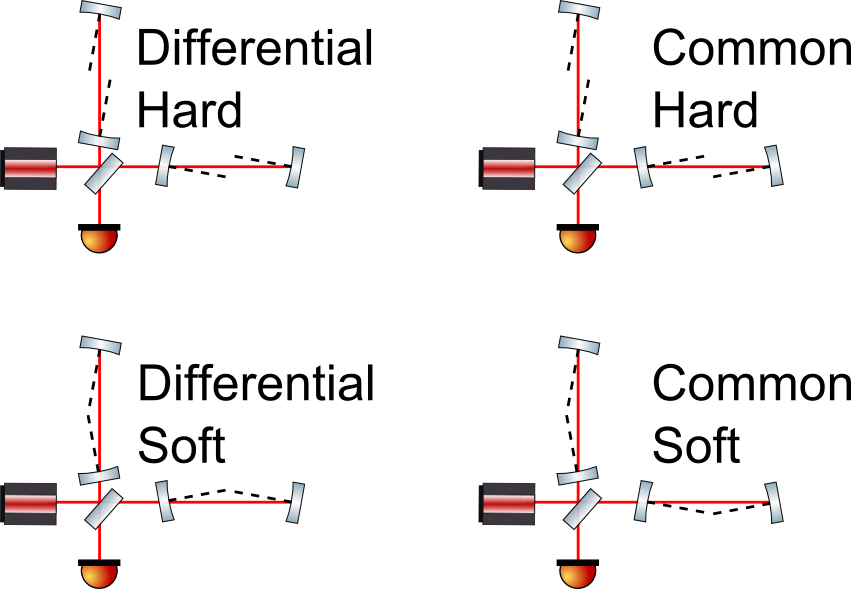
\includegraphics[width=.8\textwidth]{figures/application/SidlesSigg}%
\caption[Sidles-Sigg Modes]{The four Sidles-sigg modes of the Fabry-Perot cavities in LIGO. The two hard modes are stable and the two soft modes are unstable.}%
\label{fig:sidlessiggmodes}%
\end{figure}

Angular noise can couple in to differential arm length (DARM) though the interaction between beam spot motion (BSM) and angular motion ($\theta$) on mirrors. This happens in two ways: both a static offset in the BSM with mirror angular noise and a static angular offset with BSM noise can create DARM noise. 

\begin{equation}
\hat{\Delta L}(f) = \hat{d}_{spot}(f)*\hat{\theta}_{Mirror}(f) \approx \hat{d}_{spot}(f)*\theta_{Mirror}^{RMS}(f) + d_{spot}^{RMS}(f)*\hat{\theta}_{Mirror}(f)
\label{eq:darmcouple}
\end{equation}

Barsotti and Evans showed that, in Science Mode, angular noise from Common Soft and Differential Soft (the two modes of the arms that are unstable at high power) contribute the most to DARM noise. They also showed that in the final design of aLIGO, the soft mode is unstable with frequencies of -.17 and -.21 Hz for pitch and yaw, respectively. The optical trap will need to provide enough phase at that frequency to stabilize the mode.

Using angular trapping methods, we can reduce part of this noise contribution by damping the angular motion $\hat{\theta}_{Mirror}(f)$.

\section{Applying angular control}

For our discussion, we will disregard the distinction between common and differential modes of the interferometer.

I have considered two possible options that could (with some effort) be implemented in a LIGO-style interferometer.

\subsection{Local damping}

Damping relative to something very heavy in the end station

BSC4 layout: D0901154

Pros:

\begin{itemize}
	\item Can keep the same ETM/ITM suspensions
	\item Modular: easy to modify and/or disable
	\item Easier to build, align and lock
	\item Affects Soft and Hard modes equally.
\end{itemize}

Cons:
\begin{itemize}
  \item	Different parameters for ETM and ITM
	\item Folded Cavities
	\item worry about ISI weight limit
\end{itemize}



\begin{figure}[htp]%
\begin{center}
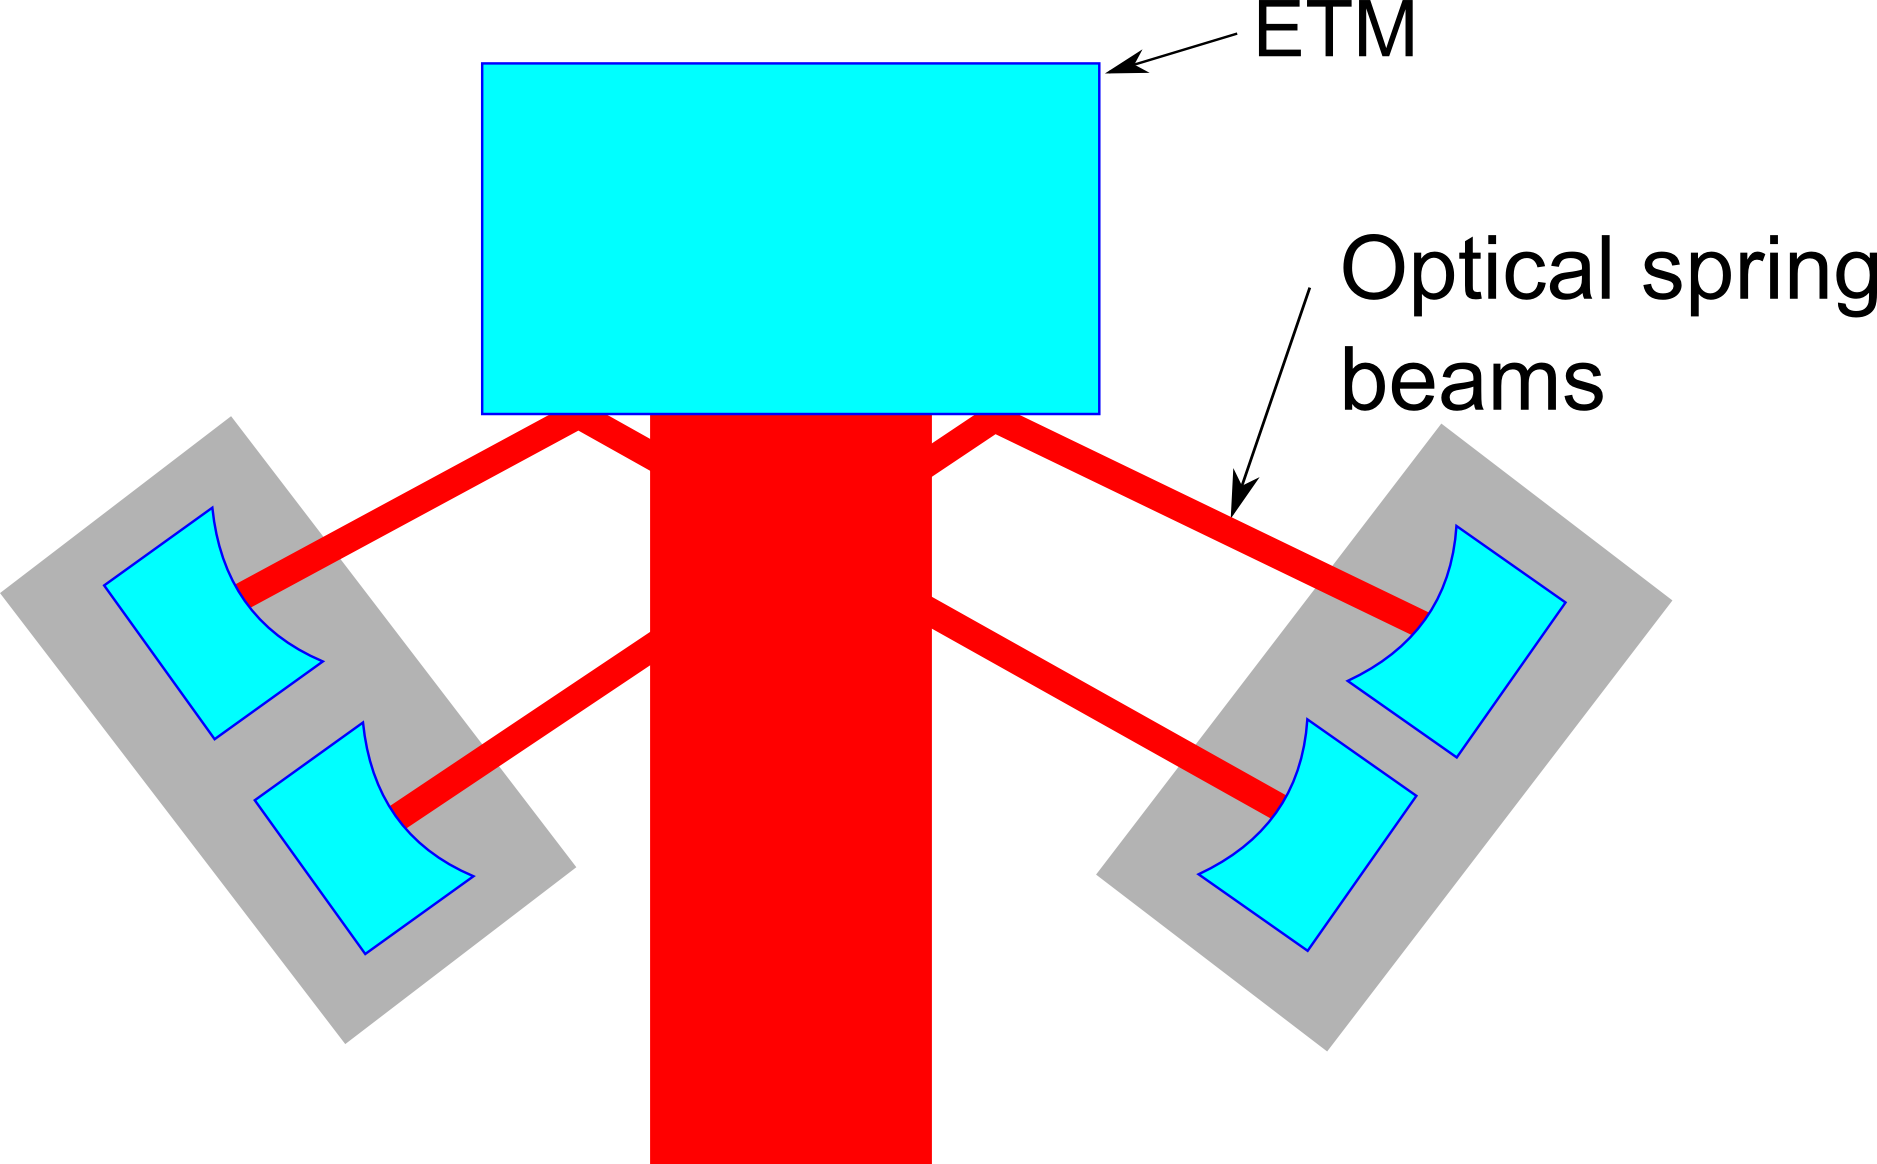
\includegraphics[width=.8\textwidth]{figures/application/shortTrapDiagram}%
\caption[Local angular control]{Diagram of a local angular control scheme. This relies on the small mirrors being mounted in something heavier than the test mass.}%
\label{fig:shorttrapdiagram}%
\end{center}
\end{figure}


\begin{table}[htp]
\centering
\begin{tabular}{ l | l | }
\bf{Parameter}& \bf{Metric}  \\ \hline
Cavity length, $L$ & 2 m \\ \hline
ETM power transmission, $T2$ & 5 ppm \\ \hline
ETM $r2$ &0.9999975 \\ \hline
ETM Diameter $D$ & 34 cm \\ \hline
ETM Thickness $t$ & 20 cm \\ \hline
Side diameter $D_s$ & 48 cm \\ \hline
Side thickness $t_s$ & 30 cm \\ \hline
Side ROC & 1.5 m \\ \hline
Cavity $FSR$ & 75 MHz \\ \hline

\end{tabular}
\caption[Local angular design]{Characteristics of proposed local angular design}
\label{tab:localproposal}
\end{table}

\begin{table}[htp]
\centering
\begin{tabular}{ l | l | }
\bf{Parameter}& \bf{Metric}  \\ \hline
Carrier Power $P_c$ & 10 W \\ \hline
Subcarrier Power $P_s$ & 2 W \\ \hline
Carrier Detuning $df_c$ & 9000 Hz \\ \hline
Subcarrier Detuning $df_s$ & -2500 Hz \\ \hline
OS Angle $\theta$ & 45 deg \\ \hline
\end{tabular}
\caption[Local angular optical springs]{Characteristics of proposed local angular optical spring}
\label{tab:localos}
\end{table}

In this design, we use radiation pressure to couple e.g. the ETM (about 40 kg) to two much larger masses (about 400 kg each) made out of stainless steel. In this fashion, we can damp the angular motion of the test mass relative to the hopefully much more stable masses on the side. 

With the control beams at \~ 45 degrees to the optical axis, we expect that the coating will be significantly lower reflectivity. Er-glass lasers at 1540 nm 

\subsection{4 km damping}

\begin{figure}[htp]%
\begin{center}
\includegraphics[width=.8\textwidth]{figures/application/longTrapDiagram}%
\caption[4 km angular control]{Diagram of a 4km angular control scheme. This relies on control mirrors attached to the side of the test mass.}%
\label{fig:longtrapdiagram}%
\end{center}
\end{figure}

Damping ETM relative to ITM. This will have significant changes because the masses of the ETM and ITM are currently the same. The angular trap we have damps the motion of one mirror by pushing on the other. In a system with equal masses, this just couples the mirrors, it doesn't damp. 

Pros:

\begin{itemize}
	\item Straight cavities
	\item Lower vacuum chamber volume
	\item Damp only Soft mode
\end{itemize}

Cons:
\begin{itemize}
	\item Does not see Hard mode motion of cavity
	\item Modify test masses and probably suspensions
	\item Hard/risky to adjust
\end{itemize}


\begin{table}[htp]
\centering
\begin{tabular}{ l | l | }
\bf{Parameter}& \bf{Metric}  \\ \hline
Cavity length, $L$ & 3994.5 m \\ \hline
ITM power transmission, $T1$ & 1.4\% \\ \hline %T0900043

ETM power transmission, $T2$ & 5 ppm \\ \hline
ITM $r1$ & 0.99298 \\ \hline
ETM $r2$ &0.9999975 \\ \hline
Cavity $FSR$ & 37.52 KHz \\ \hline
\end{tabular}
\caption{Characteristics of proposed long angular design}
\label{tab:longproposal}
\end{table}

\section{noise benefits}

The cool thing about this method is that it can work independently and in tandem with existing control systems. 

\section{path to angular damping with optical springs in aLIGO}

I think we might want to get rid of this section.